% Copyright 2004 by Till Tantau <tantau@users.sourceforge.net>.
%
% In principle, this file can be redistributed and/or modified under
% the terms of the GNU Public License, version 2.
%
% However, this file is supposed to be a template to be modified
% for your own needs. For this reason, if you use this file as a
% template and not specifically distribute it as part of a another
% package/program, I grant the extra permission to freely copy and
% modify this file as you see fit and even to delete this copyright
% notice. 

\documentclass{beamer}
\usepackage{subcaption}
\captionsetup{compatibility=false}
% There are many different themes available for Beamer. A comprehensive
% list with examples is given here:
% http://deic.uab.es/~iblanes/beamer_gallery/index_by_theme.html
% You can uncomment the themes below if you would like to use a different
% one:
%\usetheme{AnnArbor}
%\usetheme{Antibes}
%\usetheme{Bergen}
%\usetheme{Berkeley}
%\usetheme{Berlin}
%\usetheme{Boadilla}
%\usetheme{boxes}
%\usetheme{CambridgeUS}
%\usetheme{Copenhagen}
%\usetheme{Darmstadt}
%\usetheme{default}
%\usetheme{Frankfurt}
%\usetheme{Goettingen}
%\usetheme{Hannover}
%\usetheme{Ilmenau}
%\usetheme{JuanLesPins}
%\usetheme{Luebeck}
\usetheme{Madrid}
%\usetheme{Malmoe}
%\usetheme{Marburg}
%\usetheme{Montpellier}
%\usetheme{PaloAlto}
%\usetheme{Pittsburgh}
%\usetheme{Rochester}
%\usetheme{Singapore}
%\usetheme{Szeged}
%\usetheme{Warsaw}

\title{Pentocity}

% A subtitle is optional and this may be deleted
\subtitle{Group 1}

\author{Chengyu Lin \and Kailash Meiyappan \and Ying Sheng}
% - Give the names in the same order as the appear in the paper.
% - Use the \inst{?} command only if the authors have different
%   affiliation.

\institute[Columbia University] % (optional, but mostly needed)
{
  
  Columbia University}
% - Use the \inst command only if there are several affiliations.
% - Keep it simple, no one is interested in your street address.

\date{Programming and Problem Solving, Fall 2016}
% - Either use conference name or its abbreviation.
% - Not really informative to the audience, more for people (including
%   yourself) who are reading the slides online

\subject{Theoretical Computer Science}
% This is only inserted into the PDF information catalog. Can be left
% out. 

% If you have a file called "university-logo-filename.xxx", where xxx
% is a graphic format that can be processed by latex or pdflatex,
% resp., then you can add a logo as follows:

% \pgfdeclareimage[height=0.5cm]{university-logo}{university-logo-filename}
% \logo{\pgfuseimage{university-logo}}

% Delete this, if you do not want the table of contents to pop up at
% the beginning of each subsection:
\AtBeginSubsection[]
{
  \begin{frame}<beamer>{Outline}
    \tableofcontents[currentsection,currentsubsection]
  \end{frame}
}

% Let's get started
\begin{document}
\begin{frame}
  \titlepage
\end{frame}
\begin{frame}{Overview}
  \begin{itemize}
  \item
    Tools for Analysis
  \item
    Building Placement Strategy
    \begin{itemize}
        \item Pre-allocation
        \item Jigsaw Puzzle Strategy
        \item Connected Components
    \end{itemize}
  \item
    Road Construction
    \begin{itemize}
        \item Shortest Path
        \item Road Pre-building
        \item Road alongside buildings
    \end{itemize}
  \item
    Ponds and Parks
    \begin{itemize}
        \item Utility
        \item Random Walks
        \item Straight Parks and Ponds
        \item Evaluation
    \end{itemize}
  \end{itemize}
\end{frame}



\begin{frame}
  \begin{figure}
\center
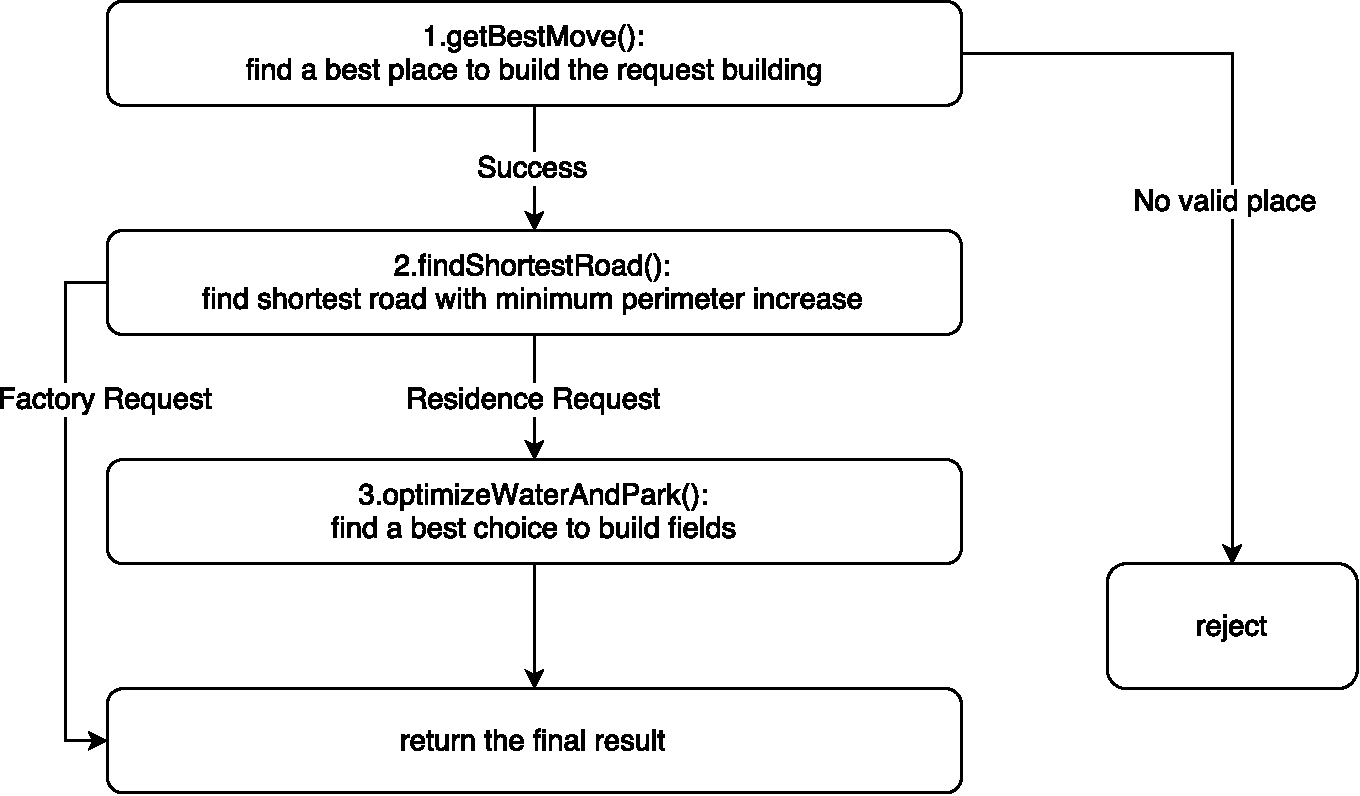
\includegraphics[scale=0.5]{pentos.pdf}
\caption{high level algorithm flow chart of our submitted approach}
\label{fig:pentos}
\end{figure}
\end{frame}

\begin{frame}
  \begin{figure}
\center

\includegraphics[scale=0.05]{pentomino.jpg}
\caption{If only the number of cells were counted, placing the U pentomino on the plus pentomino would have a score of 3, same as placing it against an edge. Counting edges gives a score of 5 versus the same 3 for an edge}
\label{fig:plusu}
\end{figure}
\end{frame}

\begin{frame}
  \begin{figure}
\center
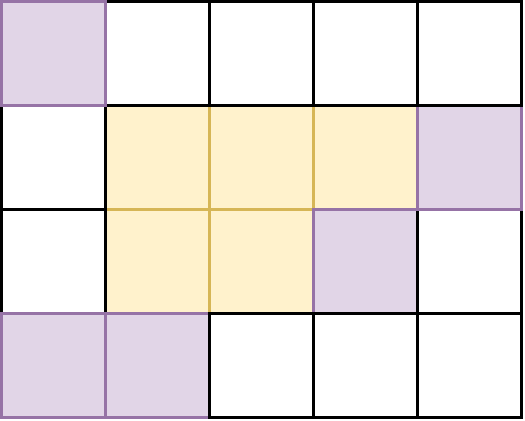
\includegraphics[scale=0.5]{numComponents.pdf}
\caption{
Suppose the yellow grids denote the candidate building place,
the purple grids denote already occupied cells,
the white grids denote vacant cells.
Then the number of components in this example is 3.}
\label{fig: numComponents}
\end{figure}
\end{frame}

\begin{frame}
  \begin{figure}
\center
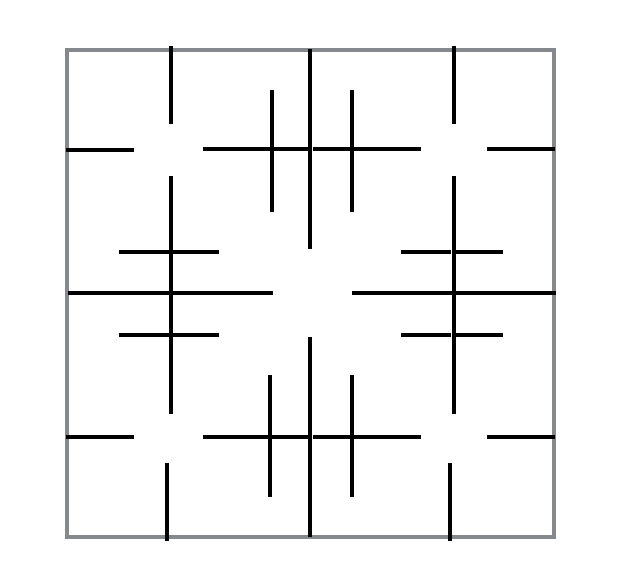
\includegraphics[scale=0.5]{prebuildRoad.png}
\caption{roads grow in fractal manner}
\label{fig: prebuildRoad}
\end{figure}
\end{frame}

\begin{frame}
  \begin{itemize}
      \item Adversarial Distribution
      \item Tournament Analysis
  \end{itemize}
\end{frame}

\begin{frame}
  \begin{figure}[ht]
\centering
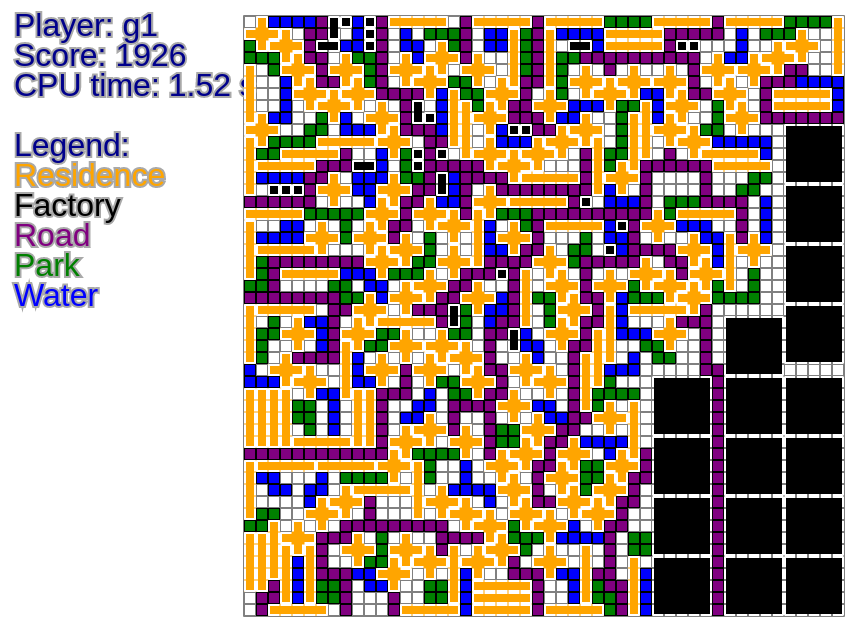
\includegraphics[width=0.8\textwidth]{IdealSolutionForAdversarial.png}
\caption{An `ideal' solution for this adversarial: let small factories
sneak into the residences area, which gives more freedom to the placement
of large factories}
\end{figure}

\end{frame}

\begin{frame}
  \begin{figure}[ht]
\centering
\begin{subfigure}[t]{.45\textwidth}
\centering
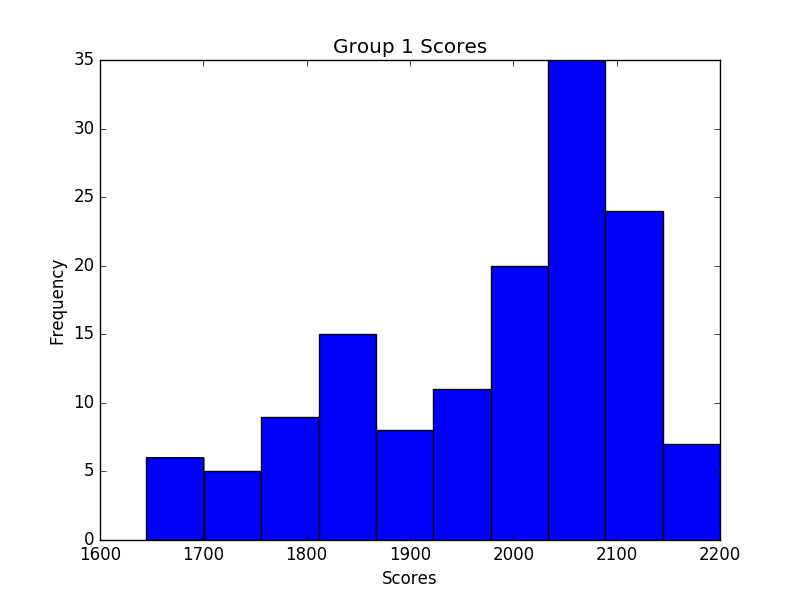
\includegraphics[width=\textwidth]{Histograms/g1.png}
\end{subfigure}
~
\begin{subfigure}[t]{.45\textwidth}
\centering
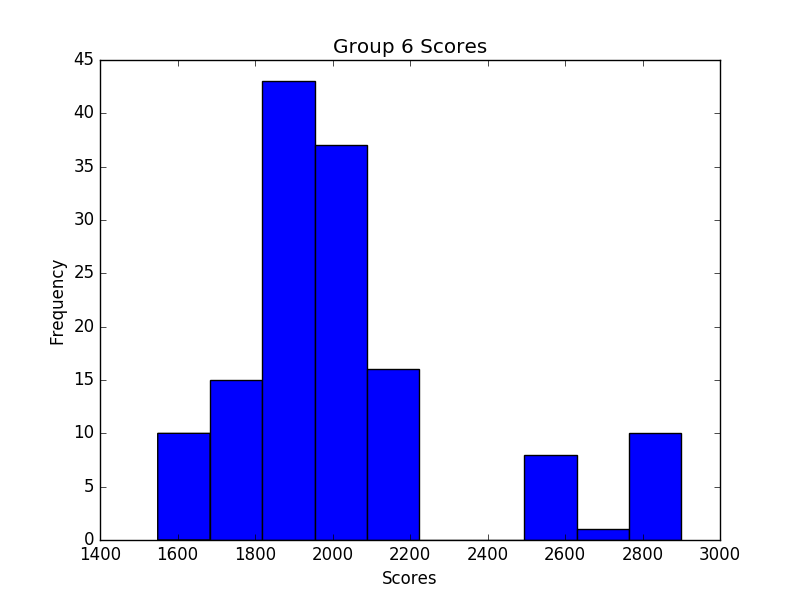
\includegraphics[width=\textwidth]{Histograms/g6.png}
\end{subfigure}
\caption{Score distribution of player 1 (left) and the highest average score player (right)}\label{fig:scores}
\end{figure}
\end{frame}



\begin{frame}
  \begin{figure}[t]
\begin{center}
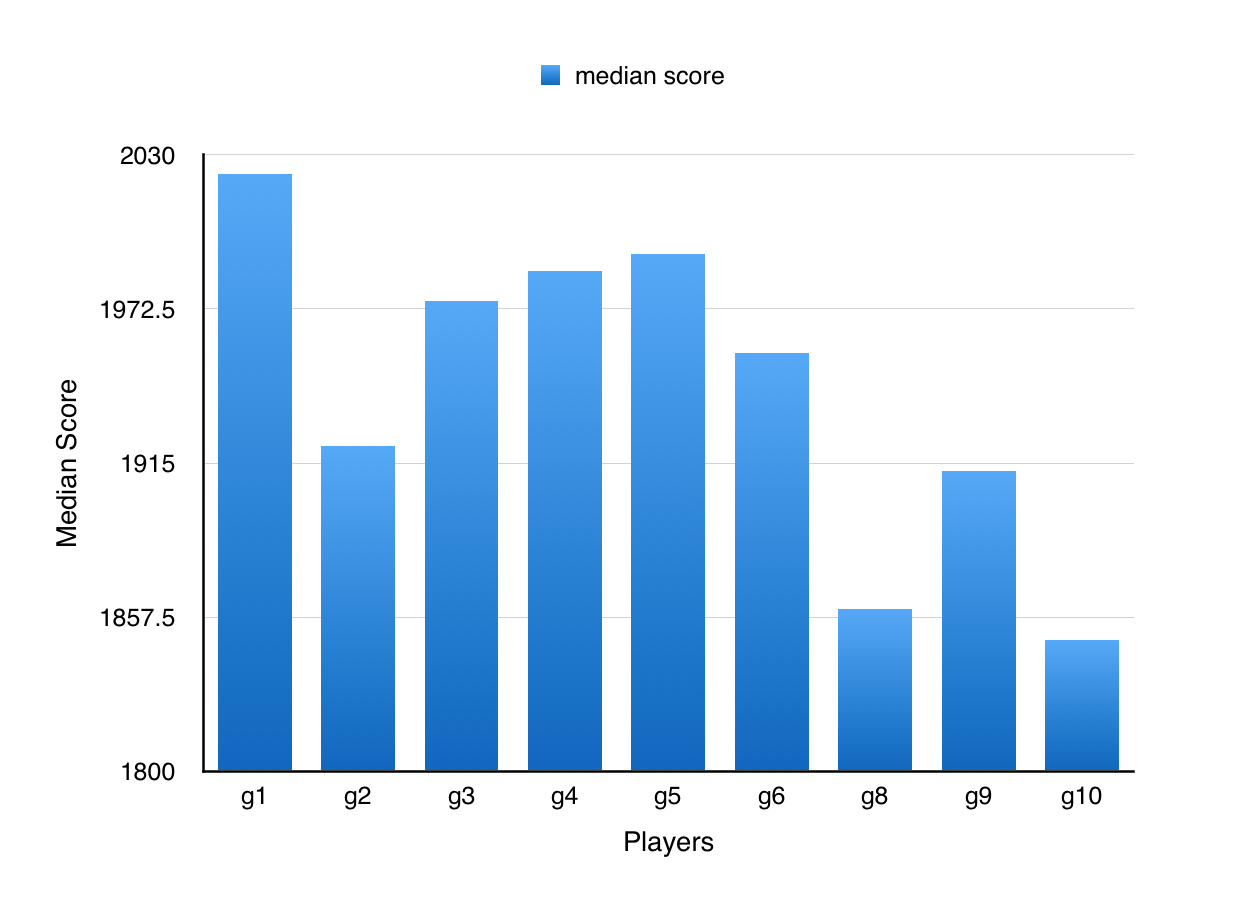
\includegraphics[width=0.48\linewidth]{median.png}
\end{center}
\caption{Median scores of each player}\label{fig:median}
\end{figure}
\end{frame}

\begin{frame}
\begin{figure}[ht]
\begin{center}
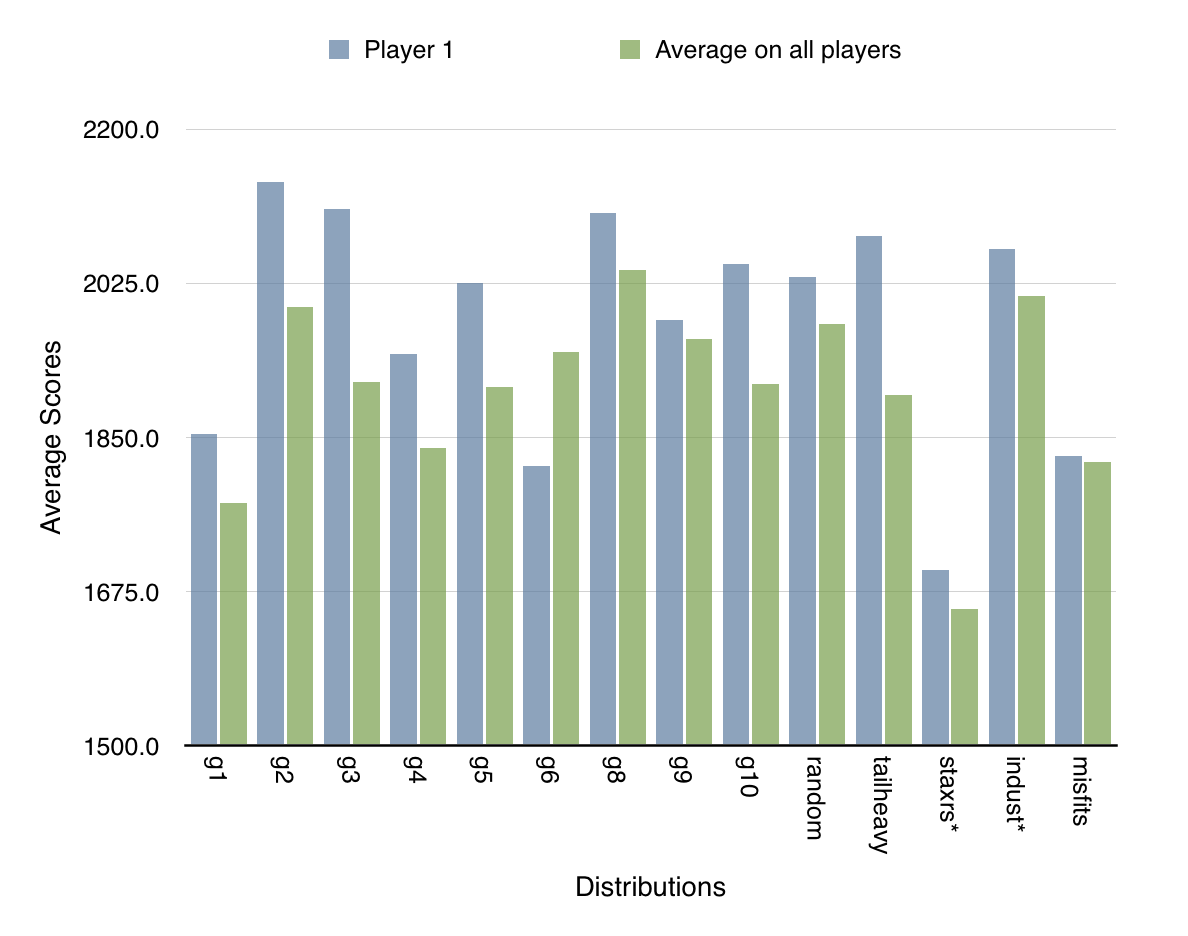
\includegraphics[width=0.48\linewidth]{average.png}
\end{center}
\caption{Averge scores of player 1 on each distribution}\label{fig:average}
\end{figure}
\end{frame}

\begin{frame}
\begin{figure}[ht]
\begin{center}
\begin{tabular}{| l | @{}c | @{}c | @{}c | @{}c | @{}c | @{}c | @{}c | @{}c | @{}c | @{}c |}
\hline
Sequencer & g1 & g2 & g3 & g4 & g5 & g6 & g8 & g9 & g10 & average \\
\hline
g1 & 1853.6 & 1784.1 & 1776.5 & 1823.4 & {\bf \color{red} 1865.8} & 1796 & 1692.5 & 1762.7 & 1621.8 & 1775.2 \\
\hline
g2 & {\bf \color{red} 2140.2} & 2005 & 2055.2 & 2043.2 & 1942 & 1948.2 & 1999.8 & 2022 & 1830 & 1998.4 \\
\hline
g3 & {\bf \color{red} 2109.2} & 1947.7 & 1410.5 & 2006.2 & 2094.4 & 1941.8 & 1722 & 2023.7 & 1961.9 & 1913.0 \\
\hline
g4 & {\bf \color{red} 1944.3} & 1872.7 & 1714.7 & 1890 & 1940.9 & 1826.6 & 1781.4 & 1823.4 & 1748.7 & 1838.1 \\
\hline
g5 & 2025.6 & 1900.3 & 1661.2 & 1963.2 & {\bf \color{red} 2120.2} & 1905.6 & 1755.2 & 1957.2 & 1872.8 & 1906.8 \\
\hline
g6 & 1817.6 & 1893.4 & 1494.1 & 2004.4 & 1943 & {\bf \color{red} 2900} & 1830.7 & 1788 & 1849 & 1946.7 \\
\hline
g8 & 2104.5 & 2030.6 & 2065.1 & 2018.5 & 2033.4 & 2046.3 & {\bf \color{red} 2140.9} & 2022.9 & 1894.5 & 2039.6 \\
\hline
g9 & 1983.6 & 1917.3 & 1713.1 & 1987.1 & 1952.3 & {\bf \color{red} 2532.3} & 1962.5 & 1809.6 & 1801.6 & 1962.2 \\
\hline
g10& {\bf \color{red} 2046.9} & 1905.7 & 1729.1 & 1923.7 & 2042.8 & 1863 & 1885.2 & 1889.4 & 1912 & 1910.9 \\
\hline
random &2031.7 & 1983 & 2067.2 & 2046.3 & 2020.1 & {\bf \color{red} 2069.9} & 1615.3 & 2029.8 & 1939.7 & 1978.1 \\
\hline
tailheavy &2078.5 & 2010.1 & {\bf \color{red} 2119.9} & 2083.9 & 2067 & 2097.3 & 615.7 & 2057.8 & 1950.3 & 1897.8 \\
\hline
stars* &1699 & 1672.4 & 1681.2 & 1697 & {\bf \color{red} 1807.2} & 1584.1 & 1656.1 & 1588.1 & 1513.2 & 1655.4 \\
\hline
indust* &2064.4 & 2001 & 2089.4 & 2029 & 2054 & {\bf \color{red} 2093.2} & 1811.6 & 2032.1 & 1915.4 & 2010.0 \\
\hline
misfits &1828.6 & 1822.8 & 1830.1 & {\bf \color{red} 1899.8} & 1778.9 & 1881.8 & 1816.2 & 1839.9 & 1703.1 & 1822.4 \\
\hline
\end{tabular}
\end{center}
\caption{Average scores of each player running on each distribution. \newline
The {\bf \color{red} bold red} ones are the distribution winner.}\label{fig:table}
\end{figure}
\end{frame}

\end{document}


